\chapter{Technologie i systemy web-GIS}
W niniejszym rozdziale zostaną przedstawione protokoły wykorzystywane podczas serwowania map, następnie zostaną omówione serwery umożliwiające przesyłanie map (GeoServer oraz MapServer).
W ostatniej części zostaną przedstawione biblioteki klienckie mogące łączyć się z serwerami i prezentujące mapy użytkownikowi.

\section{Protokoły serwowania map - WMS, WFS, WCS}
W niniejszej sekcji zostaną opisane protokoły serwowania map:
\begin{itemize}
\item WMS - Web Map Service - standard udostępniania map w postaci rastrowej za pomocą protokołu HTTP;
\item WFS - Web Feature Service - standard udostępniania danych przestrzennych w języku znacznikowym GML;
\item WCS - Web Coverage Service - standard udostępniania zmian w danych przestrzennych w czasie.
\end{itemize}

Standardy te zostały opracowane przez Open Geospatial Consortium (OCG). Jest to międzynarodowa organizacja non-profit, skupiająca się na tworzeniu wysokiej jakości standardów dotyczących systemów GIS.

\subsection{WMS}
Web Map Service jest standardem opisującym sposób udostępniania map przez serwer w postaci rastrowej za pomocą protokołu HTTP.
Zgodnie ze standardem \cite{OpenGIS_WMS2006}, rastry te mają być generowane dynamicznie na podstawie danych geograficznych.
Mapy najczęściej są zwracane w jednym z popularnych formatów graficznych, takich jak PNG, GIF lub JPG. Rzadziej jako grafika wektorowa w formatach SVG lub WebCGM.

Standard definiuje 3 dozwolone operacje: 
\begin{enumerate}
    \item GetCapabilietes - zwraca informację opisujące serwer (m.in. jego zawartość);
    \item GetMap - zwraca mapę na podstawie zdefiniowanych parametrów geograficznych;
    \item GetFeatureInfo (opcjonalna) - zwraca informację dotyczące cech obiektów, znajdujących się na mapie.
\end{enumerate}
Wszystkie te operacje mogą być wywoływane za pomocą przeglądarki internetowej poprzez URL. Parametry, które należy podać zależą od rodzaju rządania.
W przypadku prośby o dostarczenie mapy są to np: wielkość obrazka wynikowego, część Ziemi która ma zostać zobrazowana czy odwzorowanie. Pełna lista parametrów
została przedstawiona w tabeli \ref{tab:parametry_zapytania_GetMap}. Ponadto, standard dopuszcza otrzymywanie poszczególnych map z różnych serwerów.
Tym samym, WMS umożliwia stworzenie sieci rozproszonych serwerów mapowych których klienci mogą tworzyć własne mapy.

\begin{table}[h!]
    \centering
    \caption{Parametry zapytania GetMap}
    \label{tab:parametry_zapytania_GetMap}
    \begin{tabular}{|p{0.35\linewidth}|p{0.15\linewidth}|p{0.5\linewidth}|}
        \hline
        Parametr & Wymagany & Opis \\
        \hline
        VERSION=1.3.0 & Tak & Wersja serwera z którą chcemy się połączyć \\
        \hline
        REQUEST=GetMap & Tak & Nazwa rządania \\
        \hline
        LAYERS=lista\_warstw & Tak & Oddzielona przecinkami lista 1 lub więcej warstw \\
        \hline
        STYLES=lista\_styli & Tak & Oddzielona przecinkami lista styli (jednego na każdą warstwę) \\
        \hline
        CRS=system\_odniesienia & Tak & Referencyjny system odniesienia \\
        \hline
        BBOX=minx,miny,maxx,maxy & Tak & Rogi prostokąta (lewy dolny, prawy górny), który chcemy otrzymać w jednostkach wybranego systemu odniesienia \\
        \hline
        WIDTH=szerokość & Tak & Szerokość zwróconego obrazka, w pikselach \\
        \hline
        HEIGHT=wysokość & Tak & Wysokość zwróconego obrazka, w pikselach \\
        \hline
        FORMAT=format & Tak & Format zwróconego obrazka \\
        \hline
        TRANSPARENT=TRUE|FALSE & Nie & Przezroczystość tła mapy (domyślnie wyłączone) \\
        \hline
        BGCOLOR=kolor & Nie & Kolor tła w formacie heksadecymalnym (domyślnie 0xFFFFFF - biały) \\
        \hline
        EXCEPTIONS=format\_wyjątków & Nie & Format w jakim mają być zwracane wyjątki przez serwer WMS (domyślnie XML) \\
        \hline
        TIME=czas & Nie & Czas dla jakiego chcemy otrzymać mapę \\
        \hline
        Elevation=wysokość & Nie & Wysokość rządanej warstwy (np: dziura ozonowa na różnej wysokości) \\
        \hline
        Inne wymiary & Nie & Dla niektórych danych mogą być dostępne inne niż domyślne wymiary (np: podczerwone i zwykłe zdjęcia satelitarne) \\
        \hline
    \end{tabular}
\end{table}

Przykładowe zapytanie do serwera WMS wygląda następująco: 

\begin{lstlisting}[frame=single]
http://mapy.geoportal.gov.pl/wss/service/img/guest/ORTO/MapServer/WMSServer?
service=wms&
version=1.3.0&
CRS=EPSG:4326&
WIDTH=800&
HEIGHT=600&
FORMAT=image/png&
LAYERS=RASTER&
bbox=54.05,18.26,54.89,18.95&
STYLES=&
request=GetMap
\end{lstlisting}

Wynik takiego zapytania przedstawiono na rysunku \ref{fig:pomorze_gdanskie}.

\begin{figure}[h!]
    \label{fig:pomorze_gdanskie}
    \centering
    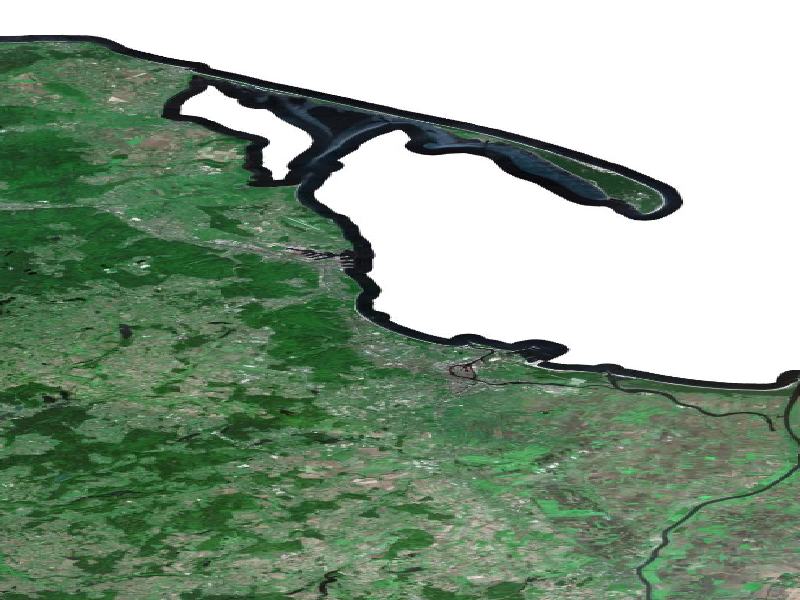
\includegraphics[width=0.7\textwidth]{img/pomorze_gdanskie.png}
    \caption{Pomorze Gdańskie zwrócone przez geoportal}
\end{figure}

\subsection{WFS}

W ostatnich latach obserwuje się rosące zapotrzebowanie na usługi oparte na danych geograficznych takie jak nawigacja \cite{TRZEBA_COS_ZNALEZC}.
W celu realizacji takich usług, konieczne jest otrzymanie mapy w formacie innym niż rastrowy czy wektorowy, w celu jej dalszego przetworzenia.
Ponadto, w dobie urządzeń mobilnych, możliwość wprowadzania poprawek do danych z dowolnego miejsca wydaje się być koniecznością.
Odpowiedzią na te dwie potrzeby jest standrad Web Feature Service.
Opisuje on, w jaki sposób przesyłać i edytować dane zapisane w metajęzyku GML za pomocą protokołu HTTP.

Metajęzyk Geography Markup Language GML jest sposobem na zapis informacji geograficznych opartym na formacie XML (formalnie rzecz biorąc, jest gramatyką dla XMLa).
Jak każda gramatyka dla XMLa, definiuje plik schematu (XML schema). Są w nim określone następujące typy węzłów:
\begin{itemize}
    \item Feature
    \item Geometry
    \item Coordinate reference system
    \item Topology
    \item Time
    \item Dynamic feature
    \item Coverage (including geographic images)
    \item Unit of measure
    \item Directions
    \item Observations
    \item Map presentation styling rules
\end{itemize}

W ramach typu \textit{geometry}, zdefiniowano 3 rodzaje geometri: punkty, linie łamane oraz wielokaty.
Ponadto, społeczności skupione wokół tych samych projektów często definiują własne typy geometryczne, takie jak drogi.
Przykładowy fragment pliku GML:

\begin{lstlisting}[frame=L, language=xml]
<gml:Point>
    <gml:posList>
        50,100
    </gml:posList>
</gml:Point>
<gml:LineString>
    <gml:posList>
        50,100 100,150
    </gml:posList>
</gml:LineString>
<gml:Polygon>
    <gml:outerBoundaryls>
        <gml:LinearRing>
            <gml:posList>
                10,10 20,10 20,20 10,20 10,10
            </gml:posList>
        </gml:LinearRing>
    </gml:outerBoundaryls>
</gml:Polygon>
\end{lstlisting}

Co więcej, GML dopuszcza także korzystanie z profili. Pozwalają one na uproszczenie tworzenia plików GML. Aby z nich skorzystać, należy je zaimportować \cite{OpeGIS_GML2007}.
Istnieje także język KML, który jest propozycją uproszczenia GMLa. Jest wykorzystywany w usługach geograficznych firmy Google \cite{kulawiak2014}.

Jak wspomniano wyżej, sposób pobierania i edytowania plików GML opisuje standard WFS. Definiuje on zestaw rządań, na które musi odpowiedzieć serwer.
Rządania te mogą być przesyłane za pomocą przeglądarki internetowej. Ponadto, standard dopuszcza używanie zapytań (query). Pozwalają one
na filtrowanie danych dostępnych na serwerze, a następnie na takim podzbiorze danych wykonanie jednego ze zdefiniowanych zapytań \cite{OpenGIS_WFS2010}.
Lista rządań prezentuje się następująco:
\begin{itemize}
    \item GetCapabilities - zwraca informacje opisujące serwer (m.in. jego zawartość);
    \item DescribeFeatureType - zwraca informacje o schematach opisujące niestandarddowe typy (np: drogi) dostępnych na danym serwerze;
    \item GetPropertyValue - informację o wartości konkretnego pola we wszystkich obiektach uzyskanych za pomocą zapytania;
    \item GetFeature - zwraca obiekty na podstawie zapytania;
    \item LockFeature - pozwala na zablokowanie dostępu do zbioru obiektów. Działa podobnie do mechanizmu blokowania znanego z relacyjnych
        baz danych.
    \item GetFeatureWithLock - podobnie jak GetFeature, lecz poza zwróceniem obiektów powienien je również zablokować;
    \item Transaction - służy do tworzenie, zmieniania, zastępowania i usuwania obiektów z serwera;
    \item CreateStoredQuery - zapisuje nowe zapytanie na serwerze;
    \item DropStoredQuery - usuwa zapytanie z serwera;
    \item ListStoredQueries - wypisuje zapytania zapisane na serwerze;
    \item DescribeStoredQueries - zwraca metadane dotyczące wszystkich zapytań zapisanych na serwerze.
\end{itemize}

Przykładowe zapytanie i odpowiedź serwera:
\begin{lstlisting}[frame=L, language=XML]
<!-- Zapytanie -->
<?xml version="1.0" ?>
<GetFeature
    version="2.0.0"
    service="WFS"
    xmlns="http://www.opengis.net/wfs/2.0"
    xmlns:fes="http://www.opengis.net/fes/2.0"
    xmlns:myns="http://www.someserver.com/myns"
    xmlns:xsi="http://www.w3.org/2001/XMLSchema-instance"
    xsi:schemaLocation="http://schemas.opengis.net/wfs/2.0.0/wfs.xsd">
    <Query typeNames="myns:InWaterA_1M">
    <wfs:PropertyName>myns:wkbGeom</wfs:PropertyName>
    <wfs:PropertyName>myns:tileId</wfs:PropertyName>
    <fes:Filter>
        <fes:ResourceId rid="InWaterA_1M.1013"/>
        <fes:ResourceId rid="InWaterA_1M.1014"/>
        <fes:ResourceId rid="InWaterA_1M.1015"/>
    </fes:Filter>
    </Query>
</GetFeature>

<!-- Odpowiedź (fragment) -->

<wfs:member>
    <InWaterA_1M gml:id="InWaterA_1M.1014">
        <wkbGeom>
            <gml:Polygon srsName="urn:ogc:def:crs:EPSG::4326" gml:id="P2">
                <gml:exterior>
                    <gml:LinearRing>
                        <gml:posList>
                        -30.92013931274414 117.6552810668945 -30.92383384704589
                        117.661361694336 -30.93005561828613 117.6666412353516
                        -30.93280601501464 117.6663589477539 -30.93186187744141
                        117.6594467163086 -30.93780517578125 117.6541137695312
                        -30.94397163391114 117.6519470214844 -30.94255638122559
                        117.6455535888672 -30.93402862548828 117.6336364746094
                        -30.92874908447266 117.6355285644531 -30.92138862609864
                        117.6326370239258 -30.92236137390137 117.6395568847656
                        -30.91708374023438 117.6433029174805 -30.91711044311523
                        117.6454467773437 -30.92061042785645 117.6484985351563
                        -30.92061042785645 117.6504135131836 -30.91638946533203
                        117.6504440307617 -30.92013931274414 117.6552810668945
                        </gml:posList>
                    </gml:LinearRing>
                </gml:exterior>
            </gml:Polygon>
        </wkbGeom>
        <id>28021</id>
        <tileId>177</tileId>
    </InWaterA_1M>
</wfs:member> 
\end{lstlisting}

\subsection{WCS}


\section{Geoserver}

\section{MapServer}

\section{OpenLayers}

\section{Leaflet.js}
